\section{RQ2 and RQ4: Models and Prediction Horizon}
\label{sec:rq2}

\subsection{Non-linear models (RQ2)}
The elastic net assumes that $\log_{10}$ life is linear in the F2 features,
i.e.\ a power law in $\mathrm{Var}(\dq)$ (life $\propto\mathrm{Var}^{-0.40}$
for F1). Section~\ref{sec:rq1} suggests where this may be too simple: the
longest-lived cells are under-predicted, and the skewness and kurtosis of
$\dq$ change sign between b1 and b2, so their effect may depend on other
features. A non-linear model must capture this from 41 cells and still
extrapolate, since some test cells lie outside the training range. Each
model maps the standardised F2 vector $\mathbf z\in\mathbb R^6$ to
$y=\log_{10}$ life.

\textbf{Gaussian process (GP).} The kernel is the linear model plus a
correction:
\begin{equation}
k(\mathbf z,\mathbf z')=\sigma_\ell^2\bigl(\sigma_0^2+\mathbf z^\top\mathbf z'\bigr)
+\sigma_m^2\Bigl(1+\sqrt5\,r+\tfrac53r^2\Bigr)e^{-\sqrt5\,r},
\label{eq:gpkernel}
\end{equation}
with $r^2=\sum_j (z_j-z'_j)^2/\ell_j^2$. The Mat\'ern term gives cells with
similar features similar corrections to the line, which can bend the power
law and couple features; a small length-scale $\ell_j$ makes feature $j$
strongly curved, a large one keeps it linear. With
$A=(K+\sigma_n^2I)^{-1}$ over the training cells and
$\mathbf k_*=k(\mathbf Z,\mathbf z_*)$,
\begin{equation}
\mu(\mathbf z_*)=\mathbf k_*^\top A\,\mathbf y,\quad
s^2(\mathbf z_*)=k(\mathbf z_*,\mathbf z_*)+\sigma_n^2-\mathbf k_*^\top A\,\mathbf k_*.
\end{equation}
Far from the training cells the correction vanishes, so the GP extrapolates
like the elastic net while $s$, and the 95\,\% interval $\mu\pm1.96s$, grow.
Parameters maximise the marginal likelihood; since the unbounded GP
interpolated the 41 cells, $\ell_j\ge1$ and noise variance $\ge0.01$ were
set by nested CV. Fitted, the correction is as large as the linear part
($\sigma_m=0.34$ vs.\ $\sigma_\ell=0.30$), five features sit near the minimum
length-scale, the skewness ($\ell=10^3$) stays linear, and the noise is at
its floor.

\textbf{Additive spline model (GAM).} The GAM lets each feature have its own
curved effect while staying readable:
\begin{equation}
\hat y=\beta_0+\sum_{j=1}^{6}f_j(z_j),\qquad
f_j(z_j)=\sum_{k=1}^{K}\beta_{jk}B_k(z_j),
\end{equation}
with cubic B-splines $B_k$ on equally spaced knots and ridge-penalised
$\beta$. It has no interactions, and beyond the training range each $f_j$
continues linearly with its slope at the edge. CV chose three knots ($K=5$,
30 coefficients for 41 cells) and ridge strength 0.03.

\textbf{Random forest (RF).} Each tree splits the cells by feature thresholds
chosen to minimise
\begin{equation}
\sum_{i:\,z_{ij}\le t}(y_i-\bar y_L)^2+\sum_{i:\,z_{ij}>t}(y_i-\bar y_R)^2
\end{equation}
and predicts the mean of a leaf; 300 bootstrapped trees are averaged. It can
find thresholds and interactions, but cannot predict outside the training
lives (300--2160 cycles). CV chose a minimum leaf of 2 cells and all features
per split.

An RBF support-vector regression (no linear term; \texttt{b1c2} at 1186) and
PLS on the whole $\dq$ curve (secondary RMSE 3431) were also dropped.

\begin{table}[!htb]
\centering
\caption{Non-linear models against the elastic net on F2: test RMSE
(cycles) / MAPE (\%). CV: nested cross-validation RMSE of $\log_{10}$ life
on the training cells. $\Delta$: RMSE change against EN-F2 with 95\,\%
bootstrap interval (negative = better); bold: interval excludes zero.}
\label{tab:rq2}
\footnotesize
\setlength{\tabcolsep}{2.6pt}
\begin{tabular}{@{}lcccc@{}}
\toprule
 & CV & Primary & In range & Secondary \\
\midrule
EN-F2  & \textbf{.0578} & 90 / 12.6 & 86 & \textbf{167} / \textbf{9.9} \\
GP-F2  & .0650 & \textbf{85} / 11.4 & 78 & 174 / 10.5 \\
GAM-F2 & .0776 & 242 / \textbf{10.6} & 79 & 169 / 14.5 \\
RF-F2  & .0951 & 188 / 14.7 & 139 & 226 / 14.5 \\
\midrule
$\Delta$ GP  & & & $-7$\,[$-35$,$+19$] & $+8$\,[$-4$,$+22$] \\
$\Delta$ GAM & & & $-8$\,[$-28$,$+14$] & $+3$\,[$-48$,$+58$] \\
$\Delta$ RF  & & & $+50$\,[$-5$,$+99$] & $\mathbf{+61}$\,[$+26$,$+99$] \\
\bottomrule
\end{tabular}
\end{table}

\textbf{Results} (Table~\ref{tab:rq2}, Fig.~\ref{fig:rq2}). Inside the
training range the GP and the GAM differ from EN-F2 by less than the
bootstrap can resolve, and both have a higher nested-CV error: 41 cells do not
support the extra flexibility. Outside it, the structure decides.
\texttt{b1c2} (2237 cycles) is predicted at 2192 by EN-F2 and 2341 by the GP,
both through their linear term, but at 742 by the GAM, whose curves turn
down near the edge of the data and continue with that slope; the two
out-of-range cells cause 90\,\% of the GAM's squared error. The RF predicts
only between 416 and 1434 cycles (\texttt{b1c2} at 1426, \texttt{b2c1} at
419) and is significantly worse on the secondary batch.

Because it fits the training cells almost exactly (training RMSE 10
cycles), the GP's interval is narrow (typically a factor of 1.16) and covers 81\,\% of the
primary and 95\,\% of the secondary cells; it widens for \texttt{b1c2}
(factor 1.84), which lies far from the training cells.

\begin{figure}[!htb]
  \centering
  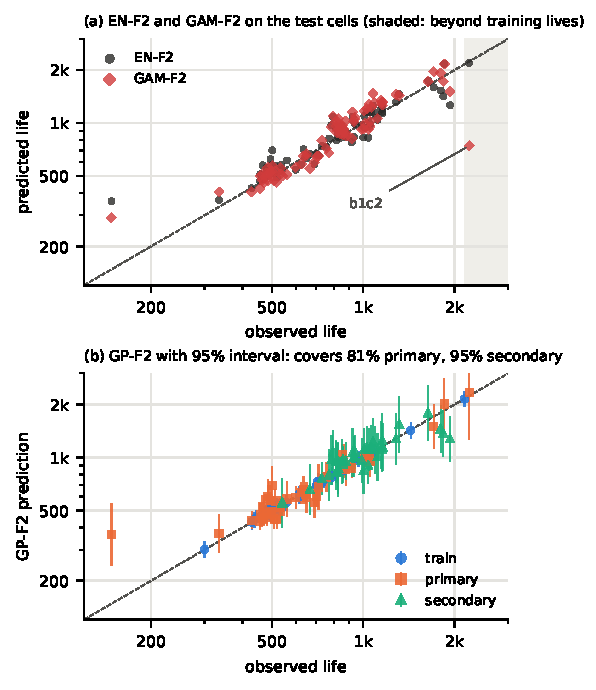
\includegraphics[width=\columnwidth]{fig_rq2_models}
  \caption{(a) EN-F2 and GAM-F2 predictions for the primary and secondary
  test cells. (b) GP-F2 predictions with 95\,\% intervals.}
  \label{fig:rq2}
\end{figure}

\textbf{Answer to RQ2.} No. With 41 training cells neither the GP nor the
GAM is significantly better than the elastic net, within the training
batches or on a new batch; the GAM fails for lives outside the training
range, and the random forest is worse everywhere.

\subsection{Number of early cycles (RQ4)}
All features were recomputed from cycles $\le N$
($\Delta Q_{N-10}(V)$, fits and minima over cycles 2--$N$,
IR($N$)$-$IR(2)) for $N=20$--150, and every model was re-tuned at each $N$.
\texttt{b2c1} (end of life at cycle 148) is excluded from the primary set
at every $N$ (Table~\ref{tab:rq4}, Fig.~\ref{fig:rq4}).

\begin{table}[!htb]
\centering
\caption{Test RMSE (cycles), primary without \texttt{b2c1} / secondary,
against the number of early cycles $N$. Life: median share of a cell's life
used by cycle $N$. F1: least squares. Constant baseline: 399 / 511. Bold:
lowest on each set.}
\label{tab:rq4}
\footnotesize
\setlength{\tabcolsep}{3pt}
\begin{tabular}{@{}rrccc@{}}
\toprule
$N$ & Life & F1 & EN-F2 & EN-F3 \\
\midrule
20  & 3\,\%  & 386 / 475 & 399 / 511 & 233 / 396 \\
30  & 4\,\%  & 324 / 335 & 306 / 350 & 205 / 345 \\
40  & 5\,\%  & 224 / 236 & 191 / 182 & 157 / 212 \\
50  & 7\,\%  & 198 / 258 & 1829 / 1186 & 168 / 247 \\
60  & 8\,\%  & 229 / 234 & 428 / 439 & 142 / 230 \\
80  & 11\,\% & 216 / 213 & 169 / 209 & 146 / 213 \\
100 & 14\,\% & 138 / 196 & 85 / \textbf{167} & 122 / 220 \\
150 & 20\,\% & 122 / 192 & \textbf{82} / 199 & 103 / 224 \\
\bottomrule
\end{tabular}
\end{table}

\begin{figure}[!htb]
  \centering
  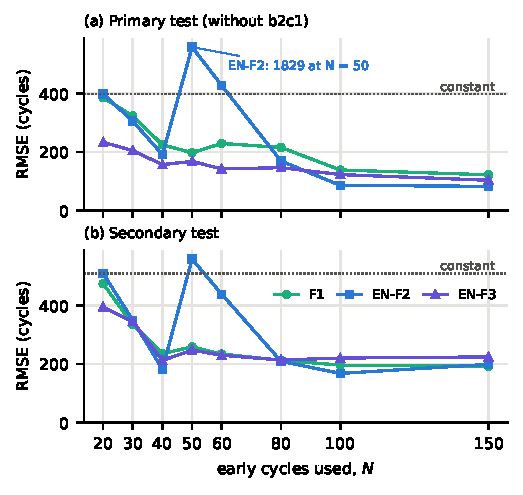
\includegraphics[width=\columnwidth]{fig_rq4_horizon}
  \caption{Test RMSE against the number of early cycles $N$ (values above
  560 clipped). Dotted: constant baseline.}
  \label{fig:rq4}
\end{figure}

\begin{itemize}
  \item \textbf{Up to 30 cycles $\Delta Q$ has no signal.} At $N=20$ the
  elastic net sets every F2 weight to zero and returns the constant, and F1
  is barely better (386 / 475); $\Delta Q_{20-10}$ is mostly noise and
  overhang release. Only F3 does better, through charge time, temperature and
  resistance, which describe the policy and batch rather than the cell; on
  the secondary set its advantage shrinks (396 vs.\ 511).
  \item \textbf{40--80 cycles} (5--11\,\% of life): F1 and EN-F3 reach about
  half the constant-baseline error; EN-F2 does at 40 and 80 cycles but fails
  at 50--60 (last point).
  \item \textbf{80 to 100 cycles: a clear drop} for F1 and F2 (EN-F2 169 to
  85 on the primary set), significant on the secondary set for EN-F2 ($-43$
  cycles). Part of this may be because the features were designed at
  $N=100$.
  \item \textbf{Beyond 100 cycles no gain.} No model improves significantly
  from 100 to 150 cycles.
  \item \textbf{The paper's log-absolute features are fragile early.} At
  $N=50$ EN-F2 predicts 13\,393 cycles for \texttt{b1c0}: its
  $\Delta Q_{50-10}$ is still near zero, so $\log_{10}|\min\Delta Q|$ lies
  8.7 standard deviations outside the training range. F1, which uses only
  the variance, has no such failure (198 / 258).
\end{itemize}

\textbf{Answer to RQ4.} About 40 cycles (5\,\% of life) are enough for a
rough screen at half the baseline error, 100 cycles are clearly better, and
more than 100 bring nothing. Below 30 cycles only policy and batch
information helps.
